\documentclass[12pt]{article}
\usepackage[a4paper,margin=1in]{geometry}
\usepackage{graphicx}
\usepackage{amsmath}
\usepackage{hyperref}
\usepackage{minted}

\begin{document}

%-------------------- Title Page --------------------
\title{Laboratory 1: Circuit Designs and Testing}
\author{Shein Htike \and Brandon Vasquez}
\date{CSC 343 Spring 2025}
\maketitle

\tableofcontents
\clearpage

\section{Exercise A: 8x1 Multiplexer Using Logic Gates}
\subsection{Objective}
The goal of this exercise is to create an 8x1 multiplexer in two ways: using logic gates and using VHDL code.
\subsection{Functionality and Specifications}
\subsubsection{Logic}
The output of the 8×1 multiplexer is given by the following logic equation:

\begin{equation}
\begin{split}
\text{output} =\,& \overline{S_2}\,\overline{S_1}\,\overline{S_0}\,I_0 \ \vee\ \overline{S_2}\,\overline{S_1}\,S_0\,I_1 \ \vee \\[1mm]
                & \overline{S_2}\,S_1\,\overline{S_0}\,I_2 \ \vee\ \overline{S_2}\,S_1\,S_0\,I_3 \ \vee \\[1mm]
                & S_2\,\overline{S_1}\,\overline{S_0}\,I_4 \ \vee\ S_2\,\overline{S_1}\,S_0\,I_5 \ \vee \\[1mm]
                & S_2\,S_1\,\overline{S_0}\,I_6 \ \vee\ S_2\,S_1\,S_0\,I_7 
\end{split}
\end{equation}

In this multiplexer design, we select one of the eight inputs, $I_{0}$ through $I_{7}$ and connect it to a single output based on the binary value of the three select signals, $S_{2}$, $S_{1}$, and $S_{0}$ (with $S_{2}$ being the most significant bit).
\clearpage
\subsubsection{Circut Design}
In order to implement the 8x1 multiplexer, we created this circuit design in Intel Quartus Prime.
This circuit was then compiled into VHDL and imported into ModelSim in order to simulate and test our design. \\
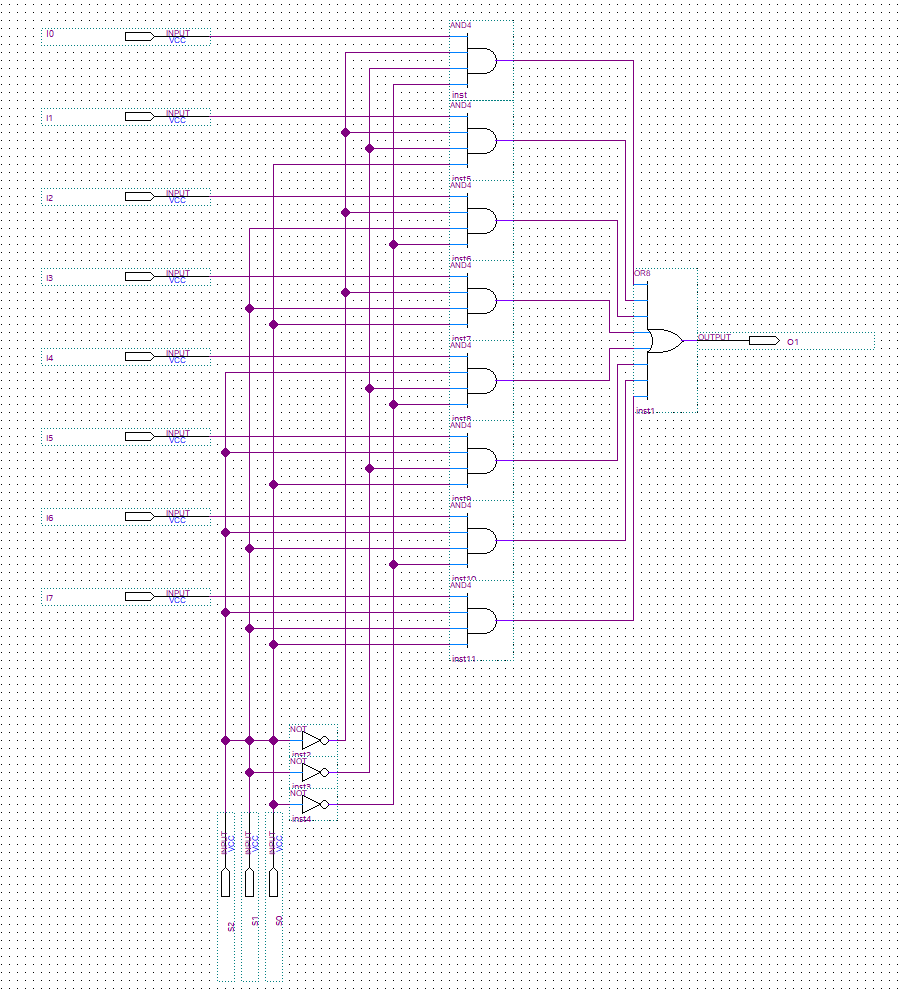
\includegraphics[width=\textwidth]{8x1multiplexer.png}
\clearpage
\subsubsection{VHDL Code}
\begin{minted}{vhdl}
    library IEEE;
    use IEEE.std_logic_1164.all;
    
    entity multiplexer8x1v2 is
        port (
            I : in  std_logic_vector(7 downto 0);
            S : in  std_logic_vector(2 downto 0);
            O : out std_logic
        );
    end multiplexer8x1v2;
    
    architecture Behavioral of multiplexer8x1v2 is
    begin
        with S select
            O <= I(0) when "000",
                 I(1) when "001",
                 I(2) when "010",
                 I(3) when "011",
                 I(4) when "100",
                 I(5) when "101",
                 I(6) when "110",
                 I(7) when "111",
                 '0'    when others;  -- Default case if needed
    end Behavioral;
\end{minted}
\clearpage

\subsection{Simulation}
\clearpage
\section{Exercise B: 1x8 De-Multiplexer Using 1x4 and 1x2 De-Multiplexers}
\subsection{Objective}

\subsection{Functionality and Specifications}

\subsection{Simulation}

\clearpage
\section{Exercise C: 3-to-8 Decoder}
\subsection{Objective}

\subsection{Functionality and Specifications}

\subsection{Simulation}

\clearpage
\section{Exercise D: 8-to-3 Priority Encoder}
\subsection{Objective}

\subsection{Functionality and Specifications}

\subsection{Simulation}

\clearpage
\section{Exercise E: Set-Reset Flip-Flop \& D Flip-Flop (Positive Edge Trigger)}
\subsection{Objective}

\subsection{Functionality and Specifications}

\subsection{Simulation}

\section{Conclusions}

\end{document}